\begin{figure*}[!htb]

    \begin{subfigure}[t]{0.48\textwidth}
        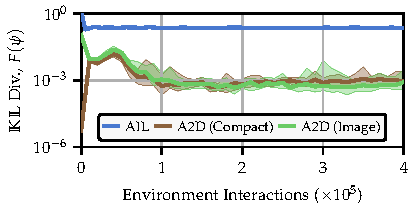
\includegraphics[width=0.95\textwidth]{figures/sec4/cr/lg/sec4_divergence_IceLake_True_cr_logs_LavaGap_LavaGapCompiledRun_.pdf}
        \caption{Frozen Lake.}
        \label{fig:grid:a2dplot:lg}
    \end{subfigure}%
    %
    \hfill%
    %
    \begin{subfigure}[t]{0.48\textwidth}
        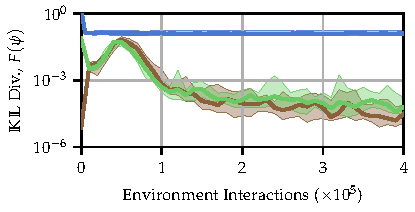
\includegraphics[width=0.95\textwidth]{figures/sec4/cr/td/sec4_divergence_TigerDoor_True_cr_logs_TigerDoor_TigerDoorCompiledRun_.pdf}
        \caption{Tiger Door.}
        \label{fig:grid:a2dplot:td}
    \end{subfigure}%
    \vspace{-0.2cm}
    \caption{The evolution of the policy divergence, $F(\psi)$.  Shown are median and quartiles across $20$ random seeds.  \emph{AIL} converges to a high divergence, whereas A2D achieves a low divergence for both representations, indicating that the trainee recovered by A2D is faithfully imitating the expert (see Figure \ref{fig:gridworld_asym} for more information). 
    { }%
    }
    \label{fig:grid:a2dplot}
\end{figure*}
